\chapter{Verificação de aderências a guideline}

A plataforma Android suporta uma grande variedades de telas e o sistema redesenha
as interfaces das aplicações de forma a preencher cada uma delas. Tipicamente, 
tudo que o desenvolvedor precisa fazer é projetar a interface para ser flexível 
e otimizar alguns elementos para telas diferentes fornecendo recursos alternativos, 
como layouts alternativos que reposicionam e/ou redefinem dimensões de alguns 
elementos. A fim de facilitar esse trabalho, no Android 3.0 (API Level 11) foi 
introduzida uma nova API: Fragments. Fragmentos permitem separar partes de uma 
interface em componentes isolados, que poderão ser combinados para criar interfaces 
com múltiplos painéis para um tablet ou “activities” separadas para um handset. 
Android 3.0 também introduziu outra API: ActionBar. ActionBar fornece um componente 
no topo da tela para identificar a aplicação e provê ações do usuário e navegação.

A documentação oficial da plataforma fornece guidelines para ajudar desenvolvedores
nessa tarefa de otimizar as aplicações para tablets e handsets\footnote{Disponível 
em http://developer.android.com/guide/practices/tablets-and-handsets.html\#Guidelines}:

\begin{itemize}
    \item{Construir a aplicação baseada em fragmentos que possam ser reutilizados 
    em diferentes combinações;}
    \item{Utilizar ActionBar, mas seguir as melhores práticas e certificar-se que 
    o design da aplicação é flexível o suficiente para o sistema ajustar o layout 
    da action bar baseada no tamanho da tela;}
    \item{Implementar layouts flexíveis.}
\end{itemize}

Neste trabalho, apresentamos uma proposta para automatizar a verificação dos dois 
primeiros itens desse guia. 

Para a nossa abordagem, definimos que os seguintes items devem ser verificados: 
\begin{itemize}
    \item{As activities deverão ser um “container” de fragmentos;}
    \item{A activity deve, de fato, estar sendo composta por fragmentos}
\end{itemize}


A partir da API Level 11, a classe {\it Activity} já suporta nativamente ser composta
por fragmentos. No entanto, na nossa abordagem iremos considerar que as activies
da aplicação deverão extender, de forma direta ou indireta, da classe FragmentActivity,
do pacote de compatibilidade V4. Assim, também garantiremos que a aplicação dará
suporte para aparelhos com versão mais antigas da API.

Para essa primeira verificação foi definido o Issue MainActivityIsFragmentActivity,
conforme figura \ref{mainactIsFragAct}.

\begin{figure}[h]
    \centering
    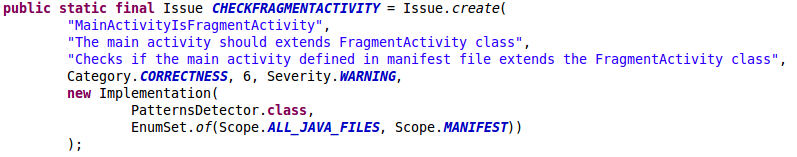
\includegraphics[width=15cm]{img/mainactIsFragAct.png}
    \caption{Definição do issue MainActivityIsFragmentActivity}
    \label{mainactIsFragAct}
\end{figure}

Caso o detector verifique que a activity não esteja fazendo a herança esperada, 
irá reportar, conforme figura \ref{activity_deve_ser_container}

\begin{figure}[h]
    \centering
    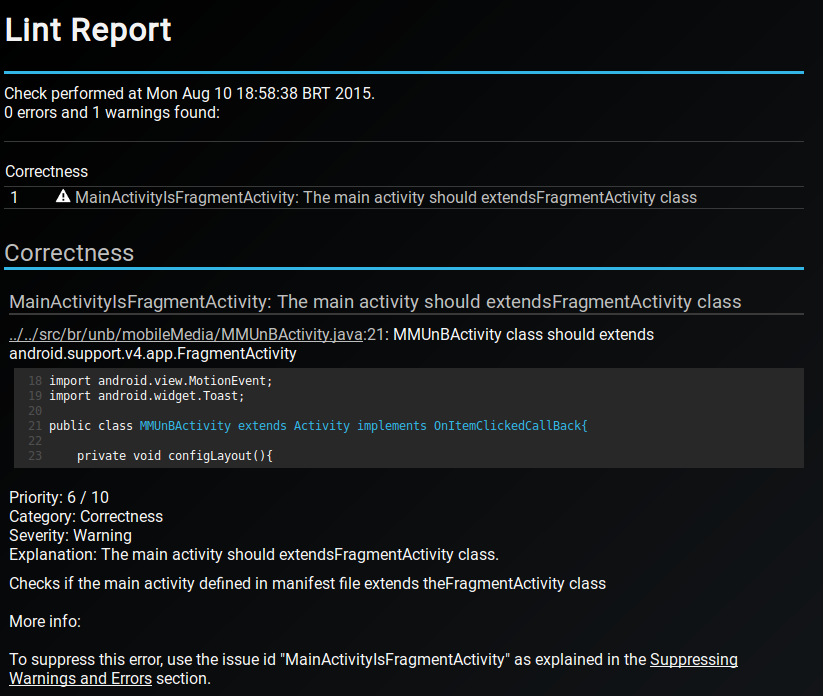
\includegraphics[width=15cm]{img/activity_deve_ser_container.png}
    \caption{Aviso de que a activity deve herdar de FragmentActivity}
    \label{activity_deve_ser_container}
\end{figure}

Para resolver esse problema, basta seguir a orientação apresentada no relatório
e fazer com que a activity {\it MMUnBActivity} herde da classe
{\it android.support.v4.app.FragmentActivity}, conforme apresentado na figura
\ref{herda_FragmentActivity}

\begin{figure}[h]
    \centering
    
\includegraphics[width=15cm]{img/heranca_FragmentActivity.png}
    \caption{Activity corretamente extendendo de FragmentActivity}
    \label{herda_FragmentActivity}
\end{figure}


